\documentclass[aspectratio=169]{beamer}
\usetheme{metropolis}           % Use metropolis theme
\title{Detonation Modeling in OpenFOAM Using Adaptive Mesh Refinement}
\date{April 29, 2020}
\author{Duncan A. McGough}
\institute{University of Colorado, Boulder \\
		{\tiny Ann and H.J. Smead Aerospace Engineering Sciences}}
\begin{document}
  \maketitle
  \begin{frame}{Overview}
    \tableofcontents
  \end{frame}

\section{Introduction}
\begin{frame}{Motivation}
\begin{columns}
\column{0.5\textwidth}
\begin{itemize}
\item Many challenges exist regarding modern combustion systems 
\item Better modeling can improve performance, efficiency, and reliability 
\item Detonation engines are a growing area of interest 
\item Current CFD models are computationally expensive
\item Adaptive meshing can reduce computational expense
\end{itemize}	

\column{0.5\textwidth}
\begin{figure}
\centering
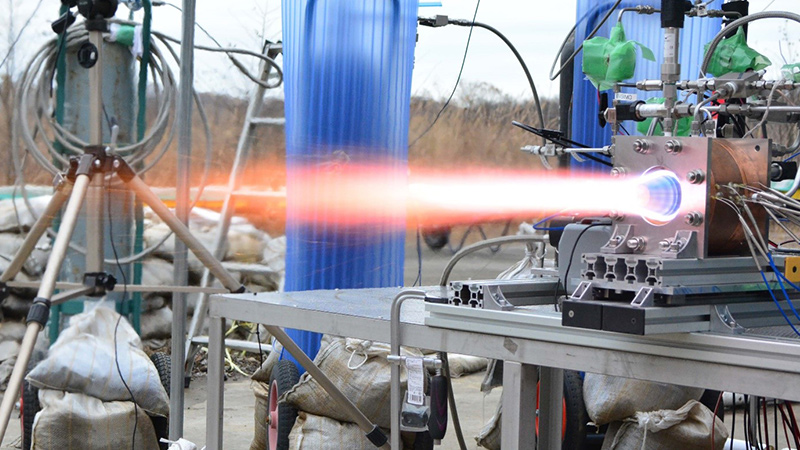
\includegraphics[width=\textwidth]{../figs/rde.jpg}
\caption{Nagoya University 900 N Rotating Detonation Engine \cite{nagoya}}
\end{figure}
\end{columns}
\end{frame}

\begin{frame}{Objectives}
\begin{itemize}
\item Implement and test AMR techniques for simulations of detonations found within RDEs and PDEs within OpenFOAM \cite{weller}
\end{itemize}
\end{frame}

  \section{AMR-Based Detonation Solver in OpenFOAM}

  \section{Solver Parameter Testing}

  \section{Summary}

\section{Bibliography}
\begin{frame}[allowframebreaks]{Bibliography}
\bibliographystyle{unsrt}	% or "siam", or "alpha", etc.
\nocite{*}		% list all refs in database, cited or not
\bibliography{../refs}		% Bib database in "refs.bib"

\end{frame}

\end{document}
